\documentclass[]{article}
\usepackage{graphicx}
\usepackage{algorithm}
\usepackage{algpseudocode}
\usepackage{amsmath, amsfonts, amssymb}

\newcommand{\abs}[1]{\left\lvert#1\right\rvert}

\title{Thiết kế và phân tích giải thuật}
\begin{document}
\maketitle{}
\section{Note:}
Giải thuật:
\begin{itemize}
\item Thời gian
\item Không gian
\item Cost
\end{itemize}
\par
Phụ thuộc:
\begin{itemize}
\item Phân cứng đi kèm
\end{itemize}
\par
$\implies$ Mỗi giải thuật có chi phí của nó, chọn giải thuật mà cho phương án cho tối ưu
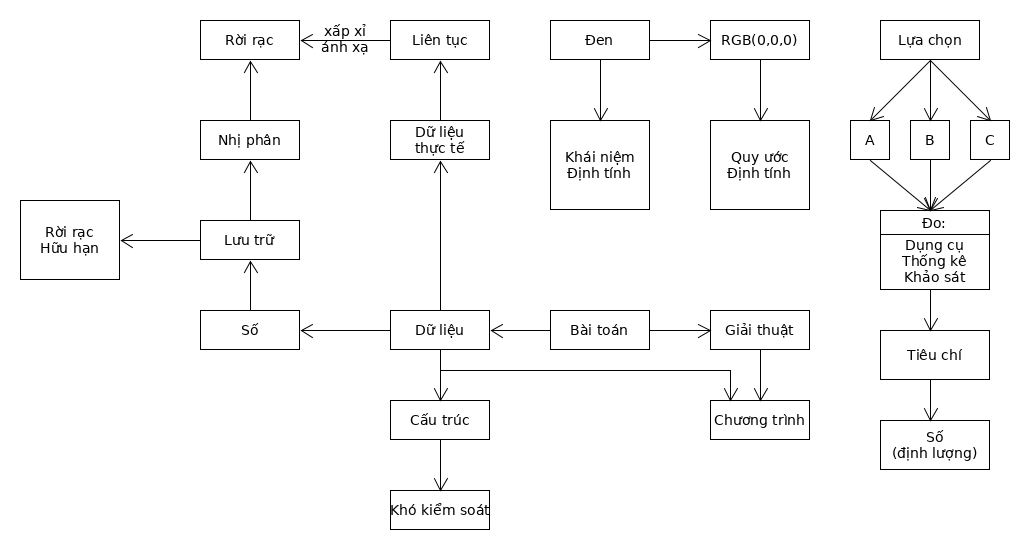
\includegraphics{intro.png}
\section{Bài tập:}
\end{document}
